\documentclass[11pt]{article}
\usepackage{amsmath}
\usepackage{amssymb}
\usepackage{tikz}
\usetikzlibrary{positioning}

\begin{document}

\begin{figure}[h]
    \centering
    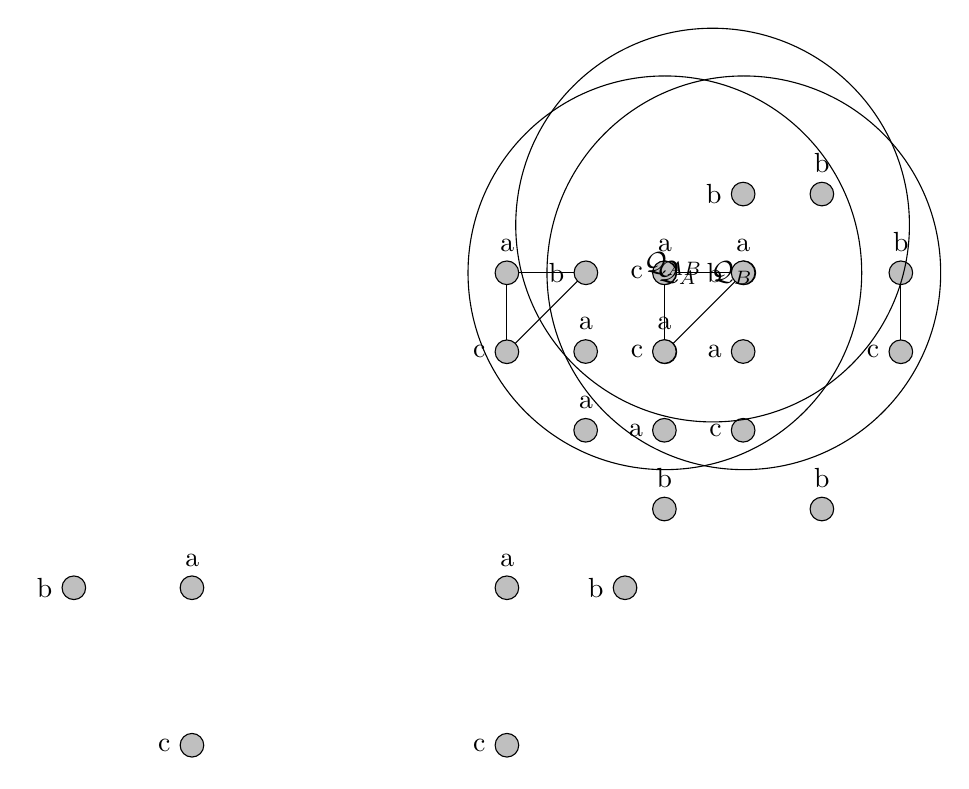
\begin{tikzpicture}[node distance=2em]
        % Define styles for nodes and circles
        \tikzset{
            dot/.style={circle, draw, fill=gray!50, minimum size=3mm},
            labeldot/.style={circle, draw, fill=gray!50, minimum size=3mm, inner sep=0pt, outer sep=0pt},
            line/.style={->, >=stealth, thick},
        }
        
        % Draw individual question sets QA and QB
        \node (qa) at (-3, 0) [labeldot,label=above:a] {};
        \node (qb) [right=of qa] [labeldot,label=left:b] {};
        \node (qc) [below=of qa] [labeldot,label=left:c] {};
        
        \draw (qa) -- (qb);
        \draw (qa) -- (qc);
        \draw (qb) -- (qc);
        
        \node [labeldot,label=above:a] at (-3, -4) {};
        \node [labeldot,label=left:b] at (-1.5, -4) {};
        \node [labeldot,label=left:c] at (-3, -6) {};
        
        \node (qb) [right=of qa, xshift=4cm] [labeldot,label=above:b] {};
        \node (qc) [below=of qb] [labeldot,label=left:c] {};
        
        \draw (qb) -- (qc);
        
        \node [labeldot,label=above:a] at (-7, -4) {};
        \node [labeldot,label=left:b] at (-8.5, -4) {};
        \node [labeldot,label=left:c] at (-7, -6) {};
        
        \node (qa) [right=of qb, xshift=-4cm] [labeldot,label=above:a] {};
        \node (qb) [right=of qa] [labeldot,label=left:b] {};
        \node (qc) [below=of qa] [labeldot,label=left:c] {};
        
        \draw (qa) -- (qb);
        \draw (qa) -- (qc);
        \draw (qb) -- (qc);
        
        \node [labeldot,label=above:a] at (0, 0) {};
        \node [labeldot,label=left:b] at (0, 1) {};
        \node [labeldot,label=left:c] at (-1, 0) {};
        \node [labeldot,label=above:b] at (1, 1) {};
        \node [labeldot,label=left:a] at (0, -1) {};
        \node [labeldot,label=above:a] at (-1, -1) {};
        \node [labeldot,label=left:a] at (-1, -2) {};
        \node [labeldot,label=left:c] at (0, -2) {};
        \node [labeldot,label=above:a] at (-2, -1) {};
        \node [labeldot,label=above:b] at (-1, -3) {};
        \node [labeldot,label=above:b] at (1, -3) {};
        \node [labeldot,label=above:a] at (-2, -2) {};
        
        % Draw circles representing QA, QB, and QAB
        \draw (qa) circle (2.5);
        \draw (qb) circle (2.5);
        \draw (qa.north east)++(0.5, 0.5) circle (2.5);
        
        % Add labels
        \node [align=center] at (qa.east) {$\mathcal{Q}_A$};
        \node [align=center] at (qb.west) {$\mathcal{Q}_B$};
        \node [align=center] at (qa.north east) {$\mathcal{Q}_{AB}$};
    \end{tikzpicture}
    
    \caption{\textit{Question Set Structure in Composite System}}
    \label{fig:question_set_structure}
\end{figure}